% !TeX spellcheck = en_US
\documentclass[a4paper,fleqn,11pt]{article}

% header
%% Packages

% Styling TOC
\usepackage{tocloft}
\setlength\cftaftertoctitleskip{1cm}
\usepackage[nottoc]{tocbibind}

% Mathe Packages
\usepackage{amsmath,amssymb,epsfig,amsthm,amsfonts,bbm,textcomp}

% Grafiken
\usepackage[font=normalsize,aboveskip=0pt,belowskip=0pt,labelfont=bf]{caption}
\captionsetup{justification=justified,singlelinecheck=false}
\usepackage[edges]{forest}
\usepackage{tikz}
\usetikzlibrary{arrows,intersections,decorations.pathreplacing}
\usepackage[utf8]{inputenc}
\usepackage[T1]{fontenc}
\usepackage{lmodern}
\usepackage[english]{babel}

% Seiten Layout
\usepackage{float}
\usepackage[top=3cm,bottom=3cm,left=3cm,right=3cm,a4paper]{geometry}
\usepackage[onehalfspacing]{setspace}
\usepackage{color}
\usepackage{enumitem}
\usepackage{authblk}

% Fussnoten
\usepackage[flushmargin,hang]{footmisc}
\usepackage{listings}
\usepackage[hyphens]{url}
\usepackage[hidelinks]{hyperref}


% Tabellen
\usepackage{longtable} 			% Lange, mehrseitige Tabelle
\usepackage{tabularx}
\usepackage{array,hhline}
\usepackage{booktabs}			% Linien zwischen Zeilen
\usepackage{multirow}			% Verknüpfte Zellen über Zeilen hinweg
\usepackage{dcolumn}			% Erlaubt variable Orientierung am Decimalpunkt innerhalb einer Zelle
\usepackage{siunitx}

% Wir brauchen auch
\usepackage{todonotes}

% References
\usepackage{natbib}

% Paragraph spacing
\setlength{\parskip}{2ex}

% Spacing around headings
\usepackage[compact]{titlesec}





\begin{document}

% title page

% header

\pagenumbering{Roman}

\title{\huge Forecasting Swiss Exports using Bayesian \\Forecast Reconciliation}

\author[$\dagger$]{Florian Eckert}
\author[$\ddagger$]{Rob J. Hyndman}
\author[$\ddagger$]{Anastasios Panagiotelis}
\affil[$\dagger$]{\small KOF Swiss Economic Institute, ETH Zurich}
\affil[$\ddagger$]{\small Department of Econometrics and Business Statistics, Monash University}
\date{July 2019}

\maketitle
\begin{abstract}
\noindent This paper conducts an extensive forecasting study on 13,118 time series measuring Swiss goods exports, grouped hierarchically by export destination and product category.  We apply existing state of the art methods in forecast reconciliation and introduce a novel Bayesian reconciliation framework. This approach allows for explicit estimation of reconciliation biases, leading to several innovations: Prior judgment can be used to assign weights to specific forecasts and the occurrence of negative reconciled forecasts can be ruled out. Overall we find strong evidence that in addition to producing coherent forecasts, reconciliation also leads to improvements in forecast accuracy.

\noindent \textbf{JEL Classification:} C32, C53, E17\\
\noindent \textbf{Keywords}: Hierarchical Forecasting, Bayesian Forecast Reconciliation, Swiss Exports, Optimal Forecast Combination.
\end{abstract}
\clearpage




% table of contents
%\tableofcontents

%\clearpage

%\listoffigures
%\listoftables

%\clearpage

\pagenumbering{arabic}

			




% 2. Model	
\section{Introduction}
\label{sec:intro}
\todo{This is more like a `background to forecast reconciliation' section rather than an intro.  We will write an intro at the end}
Data in business analytics and economics often occurs naturally in additive hierarchical structures. For instance, sales of a car dealership\todo{Can use our own motivating example} can be disaggregated by brands and then further by car model of each brand. In most cases, the series at the bottom of a hierarchy can be added up in more than one unique hierarchical way to the main aggregate. This is referred to as a grouped time series by \cite{Hyndman2016}. Retail sales for example can be added up by product type or by store location. Employment data can be aggregated by age group, gender, profession or location. Figure \ref{fig:tree} gives an example of a simple grouped hierarchy with $k = 3$ levels, $m = 9$ series in total and $q = 4$ series at the bottom.
\begin{figure}[H]
	\centering
	\begin{forest}
		before packing={
			forked edges,
		}
		[{$Y_0$}
		[{$Y_{A}$}
		[{$Y_{A1}$}]
		[{$Y_{A2}$}]
		]
		[{$Y_{B}$}
		[{$Y_{B1}$}]
		[{$Y_{B2}$}]
		]
		]
	\end{forest}\hspace{1cm}
	\begin{forest}
		before packing={
			forked edges,
		}
		[{$Y_0$}
		[{$Y_{1}$}
		[{$Y_{A1}$}]
		[{$Y_{B1}$}]
		]
		[{$Y_{2}$}
		[{$Y_{A2}$}]
		[{$Y_{B2}$}]
		]
		]
	\end{forest}
	\vspace{0.4cm}
	\caption{Simple Example of a Grouped Hierarchy}
	\label{fig:tree}
\end{figure}
All hierarchies are subject to strict aggregation constraints. In order to express the constraints in this example hierarchy, $Y_t$ is defined to be a vector containing the top-down stacked observations from all levels. $Y_{k,t}$ contains the observations at the bottom level $k$ of the hierarchy and $S$ is a corresponding aggregation matrix.
\begin{align*}
\underset{(m\times 1)}{Y_t} = \begin{bmatrix}
\ Y_0\ \ \\
\ Y_A\ \ \\
\ Y_B\ \ \\
\ Y_1\ \ \\
\ Y_2\ \ \\
\ Y_{A1}\ \ \\
\ Y_{A2}\ \ \\
\ Y_{B1}\ \ \\
\ Y_{B2}\ \ 
\end{bmatrix} \quad \underset{(m\times q)}{S} &=
\begin{bmatrix}
\ 1 & 1 & 1 & 1 \ \ \\
\ 1 & 1 & 0 & 0 \ \ \\
\ 0 & 0  & 1 & 1\ \ \\
\ 1 & 0 & 1 & 0 \ \ \\
\ 0 & 1 & 0 & 1\ \ \\
\ 1 & 0 & 0 & 0 \ \ \\
\ 0 & 1 & 0 & 0 \ \ \\
\ 0 & 0 & 1 & 0 \ \ \\
\ 0 & 0 & 0 & 1\ \ 
\end{bmatrix} \quad \underset{(q\times 1)}{Y_{k,t}} = \begin{bmatrix}
	\ Y_{A1}\ \ \\
	\ Y_{A2}\ \ \\
	\ Y_{B1}\ \ \\
	\ Y_{B2}\ \ 
\end{bmatrix} 
\end{align*}
For realized data, it must hold at each point in time that $Y_t = S Y_{k,t}$. Forecasts of the individual series however usually do not fulfill these aggregation constraints. Incoherences may arise due to model bias, varying information sets or different models used when predicting the individual series in a hierarchy. Following \cite{Gross1990}, a simple way to ensure consistency is the «bottom-up» approach. This means that only the bottom level series are forecasted and then summed up according to the hierarchical structure. It implies that forecasts from higher levels are not taken into account, even though they are usually better to predict than the noisier series at the bottom of a hierarchy. Another possibility is the «top-down» approach described in \cite{Athanasopoulos2009}, where the forecast of the top level series is disaggregated according to the historical or forecasted proportions at lower levels. This approach does not take into account the time series characteristics at lower levels. A compromise is given by the «middle-out» approach, where the forecasts at an intermediate level of the hierarchy are summed up to get the higher levels and disaggregated to obtain lower level predictions.

Many empirical studies have shown that forecast combinations improve accuracy because of information pooling and the averaging over misspecification biases and measurement errors.\footnote{See for instance \cite{Timmermann2006} or \cite{Watson2004} for a comprehensive overview.} Similarly, it is beneficial to combine information from all forecasts in a hierarchy. \cite{Hyndman2011} have shown that optimal, reconciled predictions can be obtained using the following regression approach.
\begin{align}
Y_t(h) &= S\beta_{h} + e_t(h)
\end{align}
where $Y_t(h)$ is an ($m \times 1$) vector containing the h-periods-ahead forecasts at time $t$ for each level in the hierarchy. $\beta_{h}$ represents the optimal predictions at the bottom level that minimize the deviations between the base forecasts and the consistent hierarchy. The error term $e_t(h)$ follows a normal distribution with mean zero and covariance matrix $\Sigma_h$. There is obviously a high level of heteroskedasticity in the error terms, which is why the simple ordinary least squares regression approach often leads to poor results. In order to account for this, $\beta_h$ can be estimated from a weighted least squares regression.
\begin{align}
\label{eq:reg}
\beta_{h} &= \left(S'W_h^{-1}S \right)^{-1} S'W_h^{-1}Y_t(h)
\end{align}
Intuitively, $\beta_h$ minimizes the reconciliation bias, which is the distance between actual and reconciled forecasts across the entire hierarchy. \cite{Hyndman2016} use the covariance matrix $\Sigma_h$ of the $h$-step-ahead base forecast errors as the weighting matrix $W_h$. This «GLS» approach decreases the weight of forecasts with a high prediction error in the regression. In the «MinT» approach, \cite{Wickramasuriya2015} use the covariance matrix of the $h$-step-ahead reconciled forecast errors, which they show results in the best linear unbiased reconciled forecasts. Lastly, the «nseries» approach, proposed by \cite{Athanasopoulos2017}, uses weights based on the number of series aggregated at each node.\\

This paper contributes to the literature on optimal hierarchical forecasting by constructing a Bayesian reconciliation framework that generalizes previous approaches. In section \ref{sec:model}, it introduces an explicit definition of the coherency errors as model parameters. Probabilistic reconciliation takes the uncertainty surrounding these parameters into account and leads to reconciled density forecasts. Furthermore, flexible shrinkage priors enable the model to shrink selected reconciled forecasts towards their base forecast. In section \ref{sec:appl}, the method is compared with existing reconciliation techniques using a comprehensive hierarchical dataset of Swiss goods exports.

\clearpage

\section{Bayesian Forecast Reconciliation}
\label{sec:model}
\subsection{Model}
Density forecasts have the benefit of providing additional information about the uncertainty surrounding a measure of central tendency. Recent years have seen an increase in the use of model combinations for density forecasts, such as \cite{Kapetanios2015} and \cite{Cesur2016}. In their spirit, the predictive densities of the $m$ base forecast models are approximated by drawing samples of size $n$ from the respective distributions. There are $n$ vectors $\hat{y}_{i}$ each of length $m$ that contain a draw $i$ from each predictive distribution.\footnote{Since every forecast horizon is reconciled independently, the time subscripts are dropped from now on to simplify notation.} The error term consists of two components, a prediction error $e_{i}$ and a reconciliation bias $\alpha$. The latter can be interpreted as a fixed effect that is unique to each forecasted variable. In other terms, $\alpha$ is the difference between the unreconciled forecast mean $\hat{y}$ and the reconciled forecast mean $\tilde{y}$. The interpretation of $\beta$ depends on the definition of $S$, but in general it estimates the mean of the bottom level reconciled forecasts. The following equation can then be used to model the forecast reconciliation.
\begin{align}
\label{eq:main}
\begin{tabular}{ccccccccc}
	$\hat{y}_i$ & $=$ & $\alpha$ & + &$S$ & $\times$ & $\beta$ & $+$ & $e_i$ \\
	$\scriptscriptstyle (m\times 1)$ & & $\scriptscriptstyle (m\times 1)$  & & $ \scriptscriptstyle (m\times q) $ & & $\scriptscriptstyle (q\times 1)$ & & $\scriptscriptstyle (m\times 1)$
\end{tabular}
\end{align}
where $e$ follows a normal distribution with mean zero and covariance matrix $\Sigma$. While $\Sigma$ is not singular by definition because the forecasts in $\hat{y}_{i}$ are not reconciled, it might be near-singular if the base forecasting models are estimated jointly. In the much more common case of independently estimated univariate models, $\Sigma$ is simply a diagonal matrix. The regression equation can equivalently be written as
\begin{align}
	\hat{y}_i &=  S\beta + v_i, \quad v_i \sim (\alpha,\Sigma)
\end{align}
This clarifies that a draw from the predictive distribution of any base forecast deviates from the coherent subspace either due to a unique prediction error or due to the reconciliation bias that is common to all draws from a forecasted variable. The unreconciled forecasts $\hat{y}_{i}$ follow a multivariate normal distribution. [Maybe here Tas' favourite figure?]
\begin{align}
\hat{y}\ |\ \alpha,\beta,\Sigma \sim N(\alpha + S\beta,\Sigma)
\end{align}
We are however interested in the reconciled forecasts $\tilde{y} \sim N(S\beta,\Sigma)$, which can be obtained by conditioning on $\alpha = 0$. An estimate for the reconciled means is therefore given by the conditional mean and variance functions.
\begin{align*}
E(\tilde{y}) &= E(\hat{y}|\alpha = 0,\beta,\Sigma) = \int \hat{y} f_{\hat{y}|\alpha,\beta,\Sigma}(0,\beta,\Sigma)\ d\hat{y} \\
Var(\tilde{y}) &= Var(\hat{y}|\alpha = 0,\beta,\Sigma) =  \int (\hat{y} - E(\tilde{y}))^2 f_{\hat{y}|\alpha,\beta,\Sigma}(0,\beta,\Sigma)\ d\hat{y}
\end{align*}
The reconciled conditional distribution and the corresponding moments can be retrieved conveniently from the Gibbs sampling algorithm described in the following subsection.\\

\subsection{Estimation}
To account for cross-equation correlations, the reconciliation problem in (\ref{eq:main}) can be expressed as a system of seemingly unrelated regressions. Since the explanatory variables are the same for each equation, it is a special case of the SUR model in \cite{Zellner1962}. However, the parameters are impossible to estimate directly because of perfect multicollinearity in the regressors $I_m$ and $S$. This represents an ill-posed problem because there is no unique solution. A convenient answer to this identification problem is given by Bayesian regularization methods. Following \cite{Farebrother1978}, the regression is partitioned in order to separate the parameters that cause multicollinearity. By imposing prior shrinkage on the reconciliation biases $\alpha$, it will be possible to find a unique solution to the entire estimation problem. Because of heteroskedasticity in the errors and weighting preferences introduced later, the minimization problem is given by the weighted mean squared error. The weighting matrix is given by $W = \Lambda'\Lambda$ and corresponds to $\Sigma$ in the generalized least squares case.
\begin{align}
	\frac{1}{n}\sum_{i=1}^n \Big( \Lambda^{-1}(\hat{y}_i - \alpha - S\beta)\Big)^2
\end{align}
In Bayesian statistics, data is considered to be fixed and parameters are treated as random variables. The researcher has a prior belief about the distribution of the parameters in a model. After observing the data, this prior belief is combined with the likelihood according to Bayes' theorem in order to obtain the posterior distribution of the parameters. This principle can be applied to $\alpha$, $\beta$ and $\Sigma$ in the reconciliation regression.
\begin{align}
	f(\alpha, \beta, \Sigma\ |\ \hat{y}) \propto f(\hat{y}\ |\ \alpha, \beta, \Sigma) \times f(\alpha, \beta, \Sigma)
\end{align}
In other words, the posterior distribution of the bottom-level forecasts is proportional to the likelihood of the hierarchy to be consistent times the prior distribution of the parameters. In order to approximate the distribution of $\hat{y}$, we draw $n$ $h$-periods-ahead-predictions $\hat{y}_i$ from their unreconciled predictive distributions. The likelihood function for the data is then given by 
\begin{align*}
f(\hat{y}\ |\ \alpha,\beta,\Sigma) \propto \frac{1}{|\Sigma|}\exp\left[\frac{1}{2} \sum_i \big( \Lambda^{-1}(\hat{y}_i - \alpha - S\beta)\big)'\Sigma^{-1}\big(\Lambda^{-1}(\hat{y}_i - \alpha - S\beta)\big)\right]
\end{align*}
and the posterior distribution is accordingly
\begin{align*}
f(\alpha,\beta,\Sigma,W\ |\ \hat{y}) & \propto \frac{1}{|\Sigma|^{n/2}}\exp\left[-\frac{1}{2} \sum_i \big(\Lambda^{-1}(\hat{y}_i - \alpha - S\beta)\big)'\Sigma^{-1}\big(\Lambda^{-1}(\hat{y}_i - \alpha - S\beta)\big)\right] \\
&\times \exp \left[-\frac{1}{2}(\alpha - a_0)'A_0^{-1}(\alpha - a_0)\right] \\
&\times \exp \left[-\frac{1}{2}(\beta - b_0)'B_0^{-1}(\beta - b_0)\right] \\
&\times \frac{1}{|\Sigma|(v_0 - m - 1)} \exp \left[-\frac{1}{2} tr(R_0^{-1}\Sigma^{-1}) \right]\\
&\times \frac{1}{|\Sigma|(w_0 - m - 1)} \exp \left[-\frac{1}{2} tr(Q_0^{-1}W^{-1}) \right]
\end{align*}
The Bayesian approach has the advantage that uncertainty surrounding the parameters $\alpha$, $\beta$ and $\Sigma$ is taken into account when calculating the conditional expectation of $\tilde{y}$. Following \cite{Percy1992}, we get the marginal distributions by approximating the joint posterior distribution via Gibbs sampling from the conditional distributions. After choosing a set of arbitrary starting values, the following steps are repeated until convergence. This is usually achieved very quickly, irrespective of the starting values. It can be verified by testing for stability in the recursive means of the Markov chains. After convergence is achieved, a sufficiently large sample of draws from the joint posterior is saved and evaluated. \\


\noindent\textbf{Step 1: Draw $\beta$ conditional on $\alpha,\Sigma,\hat{y},S,W$}\\
The parameter $\beta$ is the mean of the bottom level forecasts, given an appropriate aggregation matrix $S$. The conditional posterior distribution is given by
\begin{align}
\beta\ |\ \alpha,\Sigma,\hat{y} &\sim N(b_1,B_1)
\end{align}
where
\begin{align*}
B_1 &= \left(\sum_i S'W^{-1}S + B_0^{-1}\right)^{-1} \\
b_1 &= B_1 \left(\sum_i S'W^{-1} (\hat{y}_i - \alpha) + B_0^{-1}b_0\right)
\end{align*}
Unless there is reason to believe otherwise, the priors $b_0$ and $B_0$ should be chosen as uninformative as possible. In some cases, negative values in the reconciled forecasts are a concern. This issue can be resolved quite uncomplicated during the sampling process by discarding draws of $\beta$ that contain negative entries.\\

\noindent\textbf{Step 2: Draw $\Sigma$ conditional on $\alpha,\beta,\hat{y},S,W$}\\
$\Sigma$ is the covariance matrix of the prediction errors. Depending on how the draws from each predictive distribution are ordered in $Y$, there is more or less structure in the off-diagonal elements. $\Sigma$ can be drawn from an inverse Wishart distribution.
\begin{align}
\Sigma\ |\ \alpha,\beta,\hat{y} \sim W^{-1}(v_1,R_1)
\end{align}
where
\begin{align*}
v_1 &= v_0 + n\\
R_1 &=  \left( R_0^{-1} + \sum_i (\hat{y}_i - \alpha - S \beta)'(\hat{y}_i - \alpha - S \beta) \right)^{-1}
\end{align*}
It is useful to set an almost uninformative prior with $v_0$ and $R_0$ very close to zero, which introduces a tiny bit of noise into the reconciled forecasts. This has negligible impact on the posterior distribution, but ensures that $\Sigma$ is nonsingular in the case where a base forecast has no variation. If there is no correlation between the base forecast distributions, for instance if they originate from independent univariate models, it might be faster for large hierarchies to draw the variances equation-by-equation from an inverse gamma distribution.\\

\noindent\textbf{Step 3: Draw $\alpha$ conditional on $\beta,\Sigma,\hat{y},S,W$}\\
It is necessary to impose an informative prior on the reconciliation bias $\alpha$ in order to achieve identification. This process of adding information to solve an ill-posed problem is referred to as regularization\footnote{Parameter shrinkage  has been studied extensively in the literature on regularization techniques for high-dimensional data, where penalties lead to the selection of models with fewer predictors and less variance. See for instance \cite{Polson2010} for an overview.}. The conditional distribution of $\alpha$  can be obtained by concentrating out $\beta$ in the partitioned regression model. Equation (\ref{eq:prior1}) shows the basic reconciliation identity.
\begin{align}
	\label{eq:prior1}
	a &= \frac{1}{n}\sum_i \hat{y}_i - Sb
\end{align}
In order to eliminate $b$ from equation (\ref{eq:prior1}), both sides of the equation are multiplied by the projection matrix $S(S'W^{-1}S)^{-1}S'W^{-1}$. The resulting term is then subtracted from equation (\ref{eq:prior1}).
\begin{align}
	\label{eq:prior2}
	(I_m - S(S'W^{-1}S)^{-1}S'W^{-1})\ a &= (I_m - S(S'W^{-1}S)^{-1}S'W^{-1})\ \frac{1}{n}\sum_i \hat{y}_i  
\end{align}
It is useful to define the idempotent residual maker $I_m - S(S'W^{-1}S)^{-1}S'W^{-1}$ as $M$. Using $\Sigma$ as the weighting matrix $W$, the residual maker generates the generalized least squares residuals that result from a regression of the reconciliation biases on the aggregation matrix $S$. Because the generated residuals are by definition the reconciliation biases, it follows that $Ma = a$.

These simplifications leave the reconciliation biases as a function of the data, the weighting matrix $W$ and the summation matrix $S$. This result is again intuitive since the reconciliation biases are the residuals from a regression of the base forecasts on the aggregation matrix.
\begin{align}
a &= M\left(\frac{1}{n}\sum_i \hat{y}_i\right)
\end{align}
Due to the presence of multicollinearity, an inverse of the covariance matrix $A = M\Sigma M'/n$ does not exist. This issue can be resolved by introducing a tiny amount of uncertainty $A_0$  to the diagonal entries. This leads to a negligible bias, but significantly less variation in the parameter estimates. This is referred to as a ridge estimator, developed by \cite{Brown1980} and extended to the seemingly unrelated regression framework by \cite{Haitovsky1987} and \cite{Firinguetti1997}. Having enforced the orthogonality of reconciliation biases and summation matrix $S$, the prior variance $A_0$ is allowed to be uninformative. The prior mean $a_0$ is a zero vector. A numerically stable conditional posterior for $\alpha$ is therefore given by
\begin{align}
	\label{eq:alpha}
	\alpha\ |\ \beta,\Sigma,\hat{y} &\sim N(a_1,A_1)
\end{align}
where
\begin{align*}
	A_1 &= M\Bigg(\frac{\Sigma}{n}\Bigg)M' + A_0\\
	a_1 &= M\Bigg(\frac{1}{n}\sum_i \hat{y}_i\Bigg) + A_0^{-1}a_0
\end{align*}
The precision of this approach can be verified easily by comparing the estimate of $\alpha$ and the reconciliation biases from the fitted values. \\

\noindent\textbf{Step 4: Draw $W$ conditional on $\alpha,\beta,\Sigma,\hat{y},S$}\\
Using $\Sigma$ for $W$ reduces the regression to the generalized least squares estimator. Even though it is intuitive to weigh the reconciliation biases based on the predictive accuracy of the corresponding base forecasts, this can be generalized to different weighting schemes. There may exist prior information on the reliability of certain models or the requirement to fix some forecasts at specific values. This could be due to better data availability, higher suitability of a particular model or subjective judgment of the forecaster.  In this case, it is of interest to selectively shrink some reconciliation biases towards zero. At the same time, it is necessary to increase the variation of the remaining elements in $\alpha$ such that they are able to capture the increased reconciliation biases at their level of the hierarchy.

This can be achieved by keeping constant the total dispersion of a multivariate normal distribution. A common measure is the generalized variance described in \cite{Mustonen1997} and defined as the determinant of a covariance matrix. Using a diagonal scaling matrix $\lambda$ as a hyperprior on $W$, it is therefore possible to construct any weighting matrix as long as the product of the diagonal elements in $\lambda$ remain constant at 1. This in turn ensures that the total dispersion of the weighting matrix $W$ remains equal to the total dispersion of $\Sigma$. In the basic case, $\lambda$ is simply an identity matrix, which reduces $W$ to $\Sigma$. Other prior beliefs reduce some elements in $\lambda$ and increase the remaining ones. 
\begin{align}
	W\ |\ \Sigma, \lambda  \sim W^{-1}(n, n\lambda\Sigma\lambda')
\end{align}
There are several reasonable scaling methods available. A useful feature is to select certain series and shrink them towards their base forecasts. Other ossible approaches include the weighting of each series by its level in the hierarchy or by to the number of series at each node in the hierarchy. This allows for the emulation of the «nseries», «bottom-up», «middle-out» and «top-down» results. Various examples of how to shrink selected reconciliation biases are given in appendix \ref{subsec:scaling}.

\clearpage


\section{Empirical Application}
\label{sec:appl}
\subsection{Data}
We use a comprehensive dataset of exports and imports of goods in Switzerland, provided by the Swiss Federal Customs Administration. It contains the nominal value in Swiss francs of goods traded with 8 geographical regions, aggregated from 245 countries and dependent territories. In addition, the goods can be classified into economic sectors, following a national nomenclature covering 12 main groups and 48 subgroups\footnote{Precious metals, precious and semi-precious stones, works of art and antiques are generally omitted in business cycle research due to volatility and structural breaks.}. This leads to a grouped hierarchy with 13'084 time series containing nonzero entries in total. The data covers a period from 1988 to 2018 in monthly frequency and is not adjusted for seasonalities or working days. Figure \ref{fig:area} shows the composition of the regional and categorical hierarchies and their historical developments.
\begin{figure}[H]
	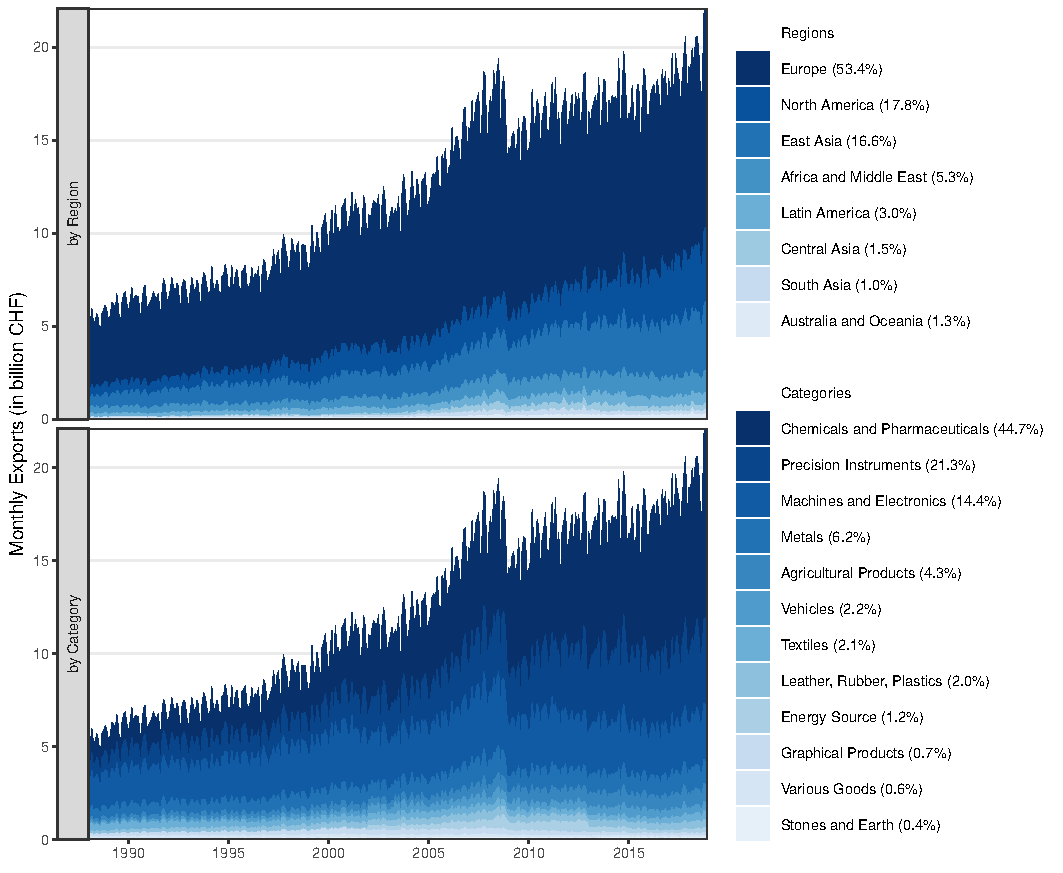
\includegraphics[width=\textwidth]{fig/fig_area}
	\caption{Regional and Categorical Contribution to Swiss Exports of Goods}\label{fig:area}
	\footnotesize{Nominal values, not seasonally adjusted. Time series range from 1988 to 2018 in monthly frequency. Average export shares of the year 2018 in parentheses.}
\end{figure}
As a result of its status as a small open economy in a rapidly globalizing world, Swiss exports have increased significantly since the late 1980s. Accounting for more than half of total exports, Europe is a key market for Swiss goods. Increasingly larger shares of exports also go to North America and East Asia with around 17\% each. Exports to Africa and the Middle East, Latin America, Central and South Asia and Australia account only for a bit more than 10\% combined.

The hierarchical grouping by categories is more evenly distributed. The most important categories are «chemicals and pharmaceuticals», «precision instruments» and «machines and electronics». Figure \ref{fig:treemap} shows the changes in composition between 1988 and 2018.
\begin{figure}[H]
	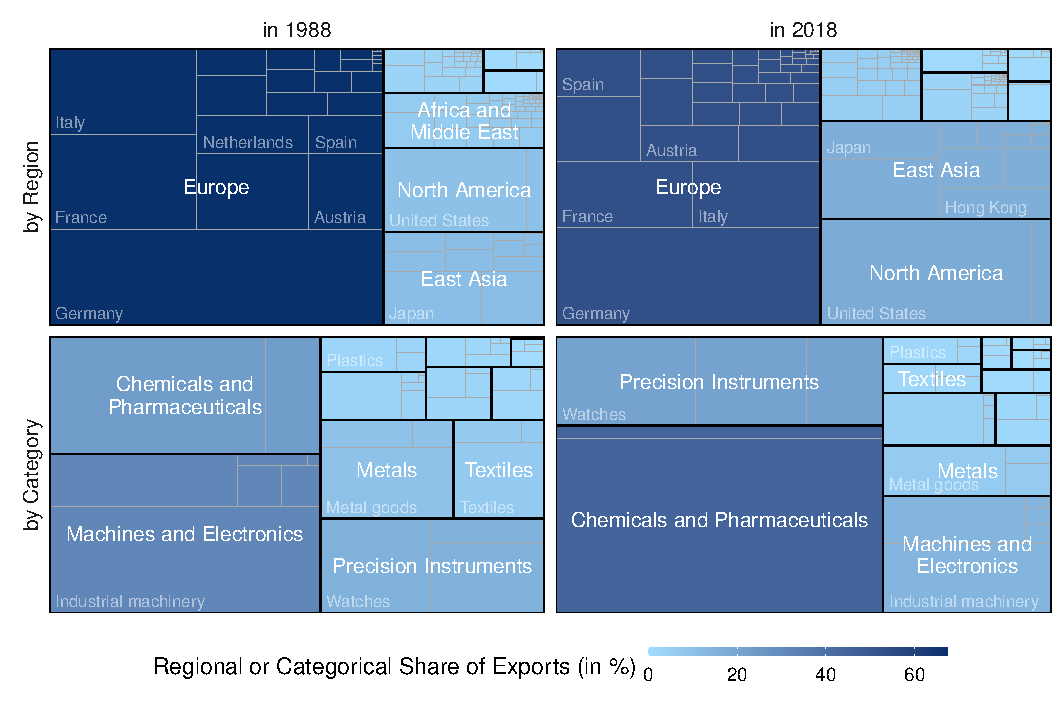
\includegraphics[width=\textwidth]{fig/fig_treemap}
	\caption{Swiss Exports in Goods}\label{fig:treemap}
\end{figure}
The two hierarchical groupings are quite different. The geographic hierarchy with 8 groups and 245 subgroups is very wide.  With a majority of the export volume going to European countries, it is nevertheless highly concentrated. In the past 30 years, the relative share of exports to the rest of the world, but especially to North America and East Asia, has increased substantially. The categorical hierarchy on the other hand is rather narrow with 12 groups and 48 subgroups. Compared to the regional hierarchy, the export volume is however more evenly distributed, even though an increasing concentration can be noted.\\

Time series at the bottom of a hierarchy are usually harder to predict than the ones at the top. Due to the aggregation involved, top level series have less observational noise and exhibit more predictable characteristics such as seasonality or trend. Following \cite{Kang2017}, it is possible to construct a measure of predictability for each time series. They estimate principal components from a number of time series features that are commonly associated with better predictability. This includes measures such as the strength of seasonality, trend, spectral entropy and serial correlation. Figure \ref{fig:feature} shows the first principal component, which accounts for a large share of the variation in these predictability features.
\begin{figure}[H]
	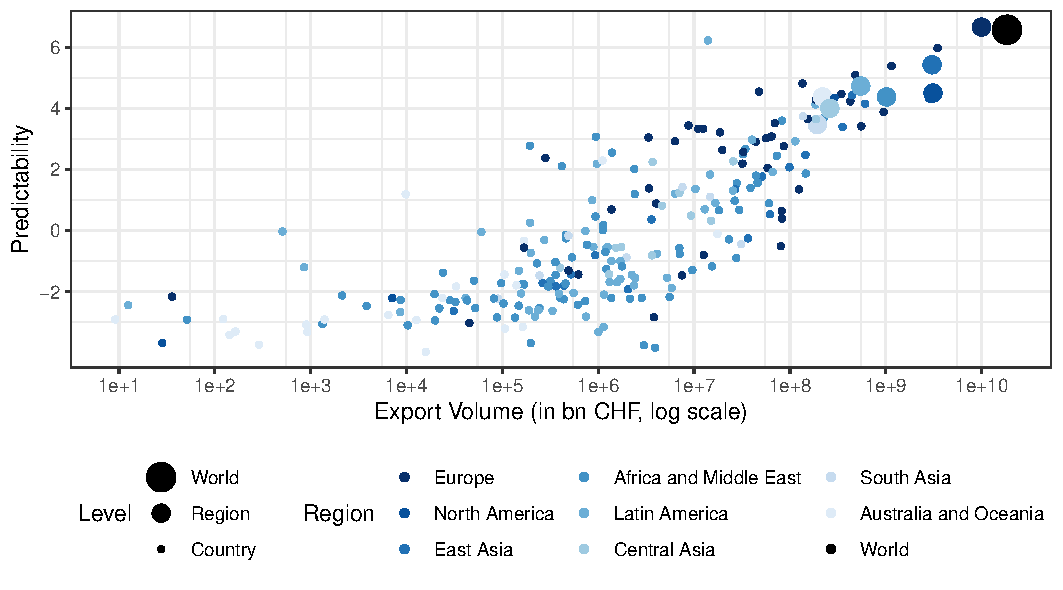
\includegraphics[width=\textwidth]{fig/fig_confetti}
	\caption{Predictability of Different Levels in a Hierarchy} \label{fig:feature}
	\footnotesize{Predictability is calculated as the first principal component of extracted time series features such as trend, strength of seasonality, spectral entropy and first order autocorrelation.}
\end{figure}
It is evident that there exists a strong correlation between predictability and export volume. This implies that larger series and consequently the series at the top of a hierarchy will be easier to forecast. This finding affirms the claim, that the reconciliation biases for top level series should be relatively smaller than those at the bottom level.

\clearpage

\subsection{Preliminary Results}
This section will answer questions w.r.t to the benefits of reconciliation/combination over unreconciled forecasting, which reconciliation methods work particularly well and which series and time periods benefit more from reconciliation.\\
 
 Is it beneficial to use hierarchies instead of unreconciled forecasts?
 \begin{figure}[H]
 	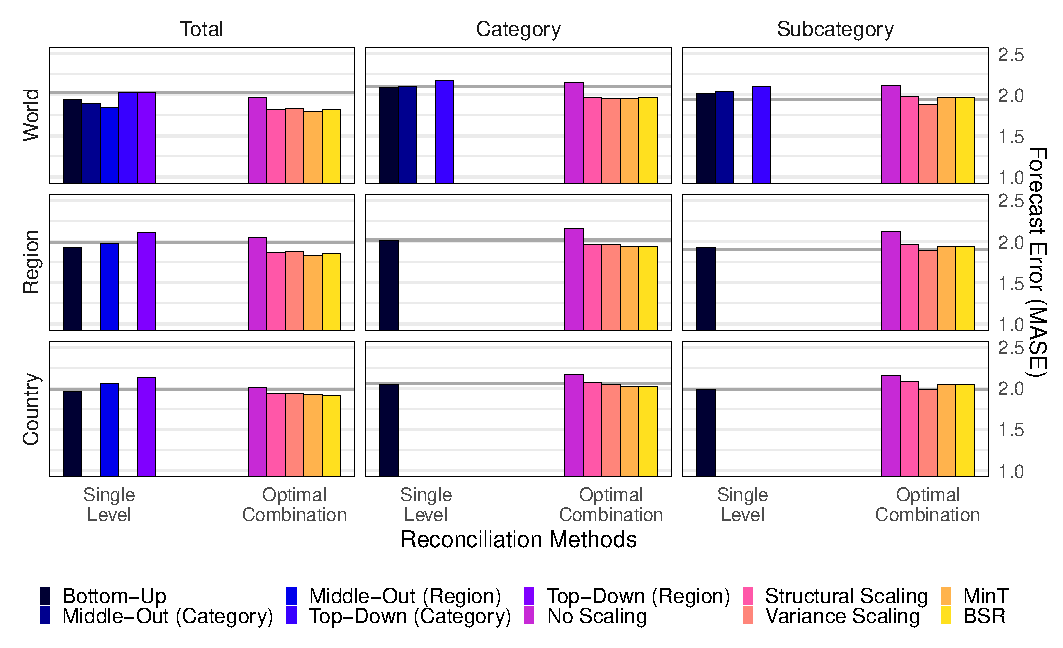
\includegraphics[width=\textwidth]{fig/fig_eval_mase}
 	\caption{Accuracy of Reconciliation Methods at Different Levels}
 	\footnotesize{Average of all time periods, forecasting horizons and methods. Lower level forecast errors are weighted by their respective export share.}
 \end{figure}

Which reconciliation procedures produce the best forecasts?
 \begin{figure}[H]
	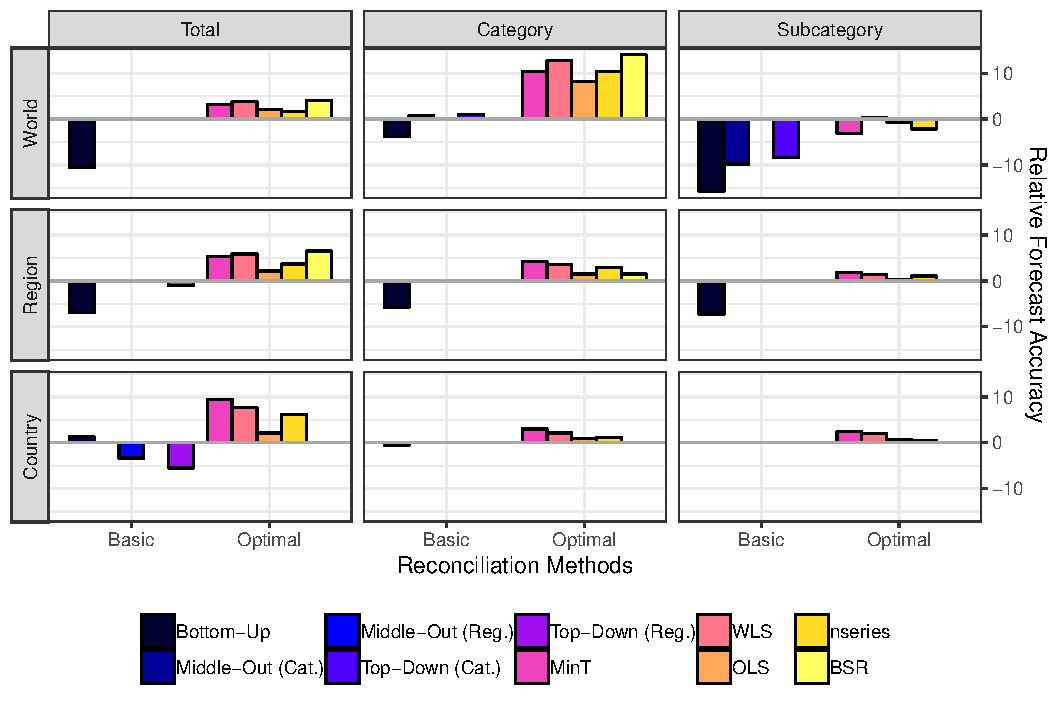
\includegraphics[width=\textwidth]{fig/fig_eval_rmse_relative}
	\caption{Accuracy of Reconciliation Methods at Different Levels}
	\footnotesize{Average of all time periods, forecasting horizons and methods. Lower level forecast errors are weighted by their respective export share.}
\end{figure}
In which periods of time was reconciliation particularly useful?
 \begin{figure}[H]
	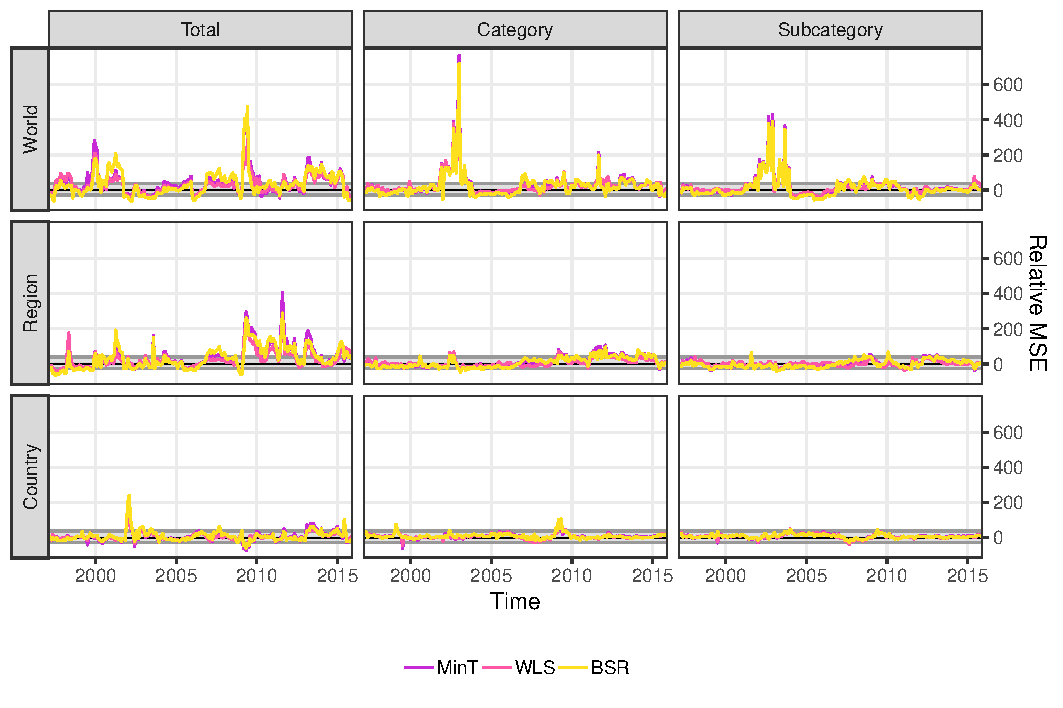
\includegraphics[width=\textwidth]{fig/fig_eval_rmse_time}
	\caption{Accuracy of Reconciliation Methods at Different Levels}
	\footnotesize{Average of all time periods, forecasting horizons and methods. Lower level forecast errors are weighted by their respective export share.}
\end{figure}
For which series in a hierarchy is reconciliation particularly useful?
 \begin{figure}[H]
	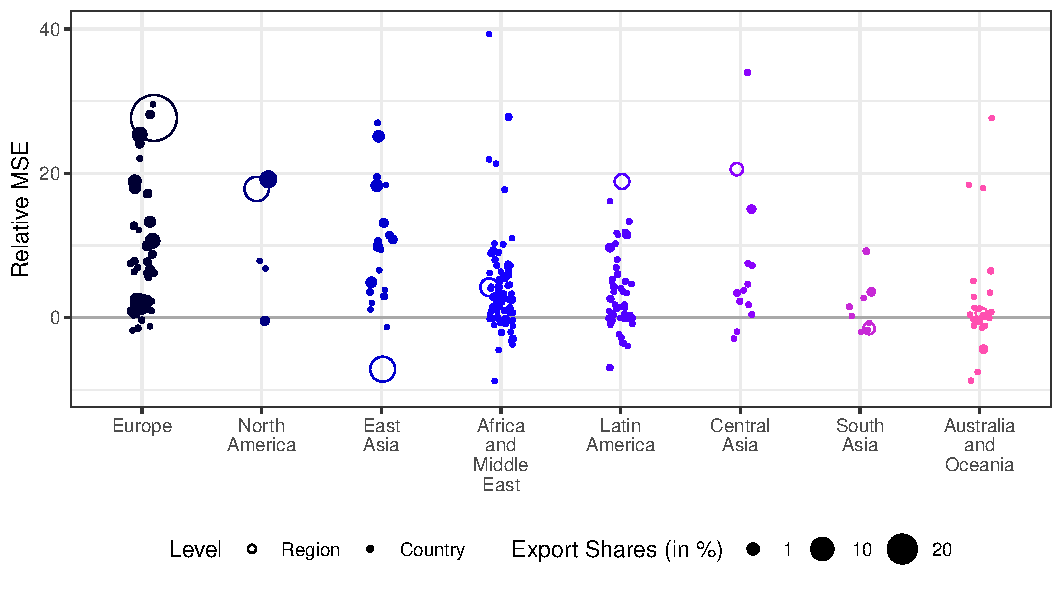
\includegraphics[width=\textwidth]{fig/fig_eval_regions}
	\caption{Accuracy of Reconciliation Methods at Different Levels}
	\footnotesize{Average of all time periods, forecasting horizons and methods. Lower level forecast errors are weighted by their respective export share.}
\end{figure}

 \begin{figure}[H]
	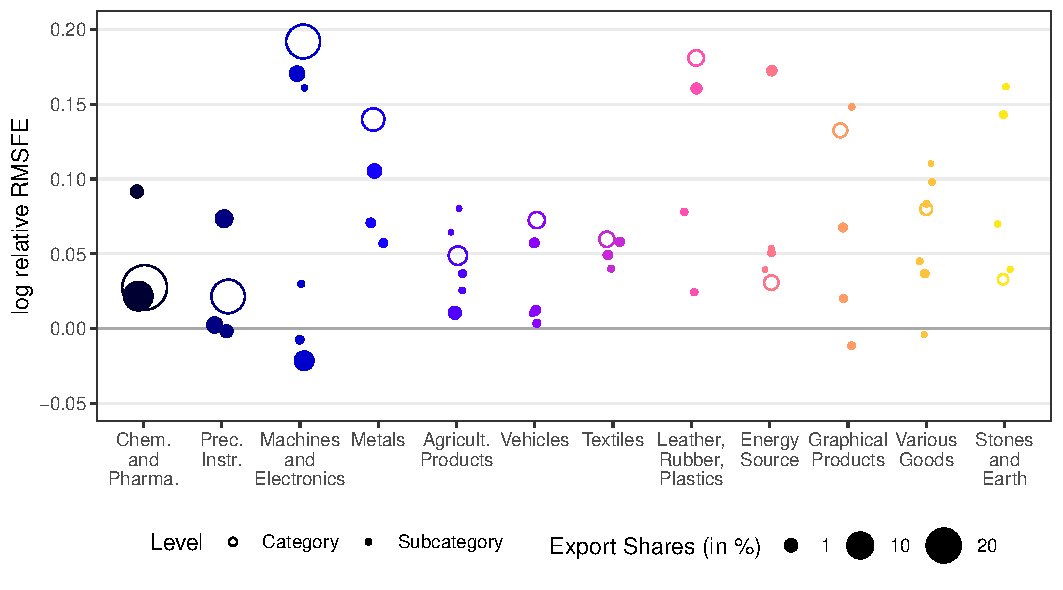
\includegraphics[width=\textwidth]{fig/fig_eval_categories}
	\caption{Accuracy of Reconciliation Methods at Different Levels}
	\footnotesize{Average of all time periods, forecasting horizons and methods. Lower level forecast errors are weighted by their respective export share.}
\end{figure}
 
 Todo:
 \begin{itemize}
 	\item  Plot with density forecast for main category (e.g.World) and subcategory (e.g. Australia)
 	\item Forecast experiment with downweighted euro area forecasts during the Swiss franc shock 2015
 \end{itemize}


\clearpage

\section{Conclusion}







\clearpage

% bibliography
\pagenumbering{Roman}
\setcounter{page}{3}
\bibliography{library}
\bibliographystyle{apalike}

\clearpage


% appendix

\appendix
\section{Appendix}


\subsection{Robustness}
\label{sec:robust}

\begin{figure}[H]
	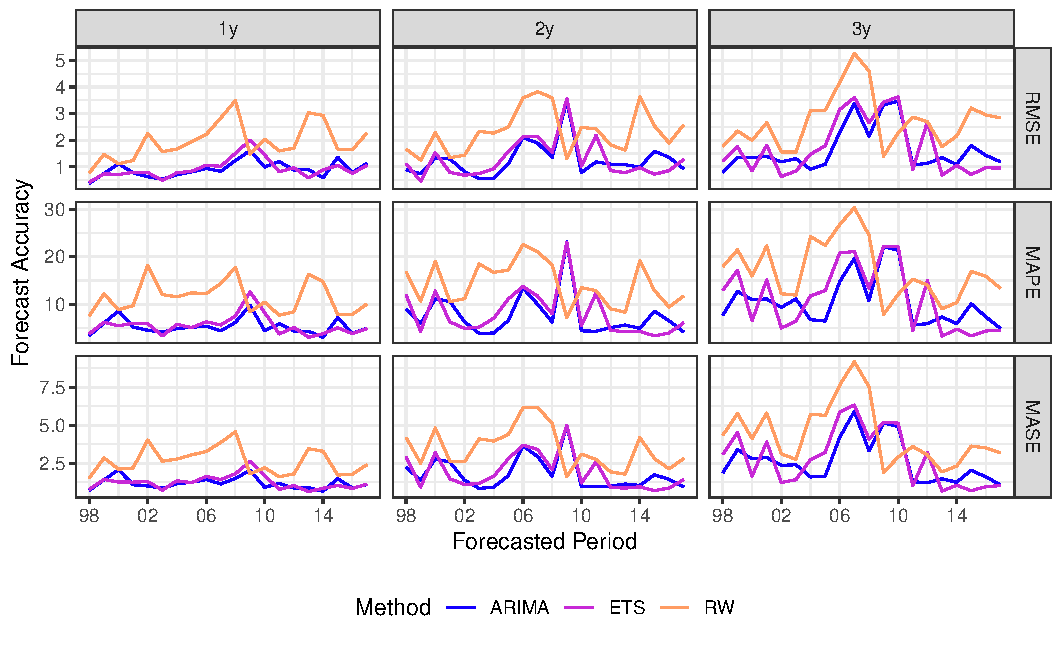
\includegraphics[width=\textwidth]{fig/fig_eval_methods_top}
	\caption{Accuracy of Forecasting Methods at the Top Level}
\end{figure}

\begin{figure}[H]
	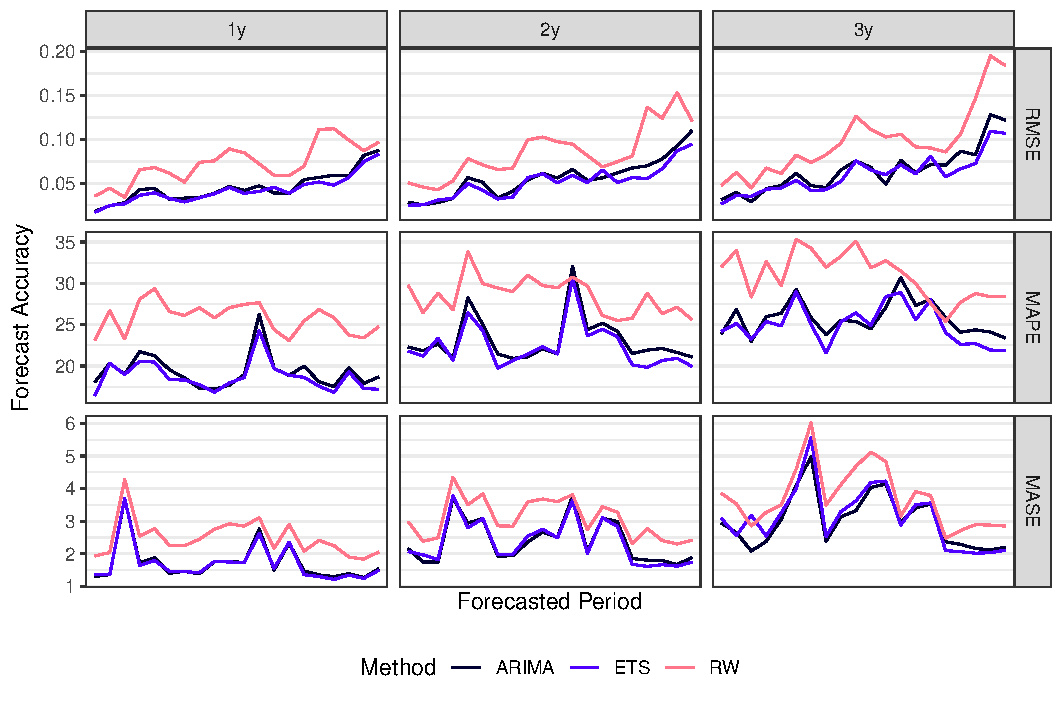
\includegraphics[width=\textwidth]{fig/fig_eval_methods_bottom}
	\caption{Accuracy of Forecasting Methods at the Bottom Level}
\end{figure}


\subsection{Data}
\label{sec:data}
The data is compiled by the Swiss Federal Customs Administration\footnote{\url{https://www.ezv.admin.ch/ezv/en/home/topics/swiss-foreign-trade-statistics.html}} and made available in a machine-friendly format on basis of a subscription.\\
% table with goods categories
\begin{small}
\begin{longtable}{p{2.5cm}p{11.5cm}}
\caption{Tariff Numbers and Descriptions of Goods}\\
\toprule
\normalsize{Tariff Number} & \normalsize{Description}\\
\midrule
\endfirsthead
\multicolumn{2}{@{}l}{\ldots continued}\\
\toprule
\normalsize{Tariff Number} & \normalsize{Description}\\  
\midrule
\endhead
\bottomrule
\multicolumn{2}{r@{}}{continued \ldots}\\
\endfoot
\bottomrule
\endlastfoot
	01	&	Forestry and agricultural products, fisheries	\\
\enskip	01.1	&	Food, beverages and tobacco	\\
\enskip	01.2	&	Feeding stuffs for animals	\\
\enskip	01.3	&	Live animals	\\
\enskip	01.4	&	Horticultural products	\\
\enskip	01.5	&	Forestry products (not firewood)	\\
\enskip	01.6	&	Products for commercial/industrial further processing such as oils, fats, starches, plants and vegetable parts, etc.	\\
\midrule
	02	&	Energy source	\\
\enskip	02.1	&	Solid combustibles	\\
\enskip	02.2	&	Petroleum and distillates	\\
\enskip	02.3	&	Gas	\\
\enskip	02.4	&	Electrical energy	\\
\midrule
	03	&	Textiles, clothing, shoes	\\
\enskip	03.1	&	Textiles	\\
\enskip	03.2	&	Articles of apparel and clothing	\\
\enskip	03.3	&	Shoes, parts and accessories	\\
\midrule
	04	&	Paper, articles of paper and and products of the printing industry	\\
\enskip	04.1	&	Basic materials for paper production, such as cellulose and cellulose fibre and paper and carton waste	\\
\enskip	04.2	&	Paper and carton in rolls, strips or sheets	\\
\enskip	04.3	&	Goods from paper or carton	\\
\enskip	04.4	&	Products of the printing industry	\\
\midrule
	05	&	Leather, rubber, plastics	\\
\enskip	05.1	&	Leather	\\
\enskip	05.2	&	Rubber	\\
\enskip	05.3	&	Plastics	\\
\midrule
	06	&	Products of the chemical and pharmaceutical industry	\\
\enskip	06.1	&	Chemical raw materials, basic materials and unformed plastics	\\
\enskip	06.2	&	Chemical end products, vitamins, diagnostic products, including active substances	\\
\midrule
	07	&	Stones and earth	\\
\enskip	07.1	&	Mineral raw materials and basic products	\\
\enskip	07.2	&	Goods from stone and cement	\\
\enskip	07.3	&	Ceramic wares	\\
\enskip	07.4	&	Glass	\\
\midrule
	08	&	Metals	\\
\enskip	08.1	&	Iron and steel	\\
\enskip	08.2	&	Non-ferrous metals	\\
\enskip	08.3	&	Metal goods	\\
\midrule
	09	&	Machines, appliances, electronics	\\
\enskip	09.1	&	Industrial machinery	\\
\enskip	09.2	&	Agricultural machines	\\
\enskip	09.3	&	Household appliances	\\
\enskip	09.4	&	Office machines	\\
\enskip	09.5	&	Electrical and electronic industry appliances and devices	\\
\enskip	09.6	&	Military equipment	\\
\midrule
	10	&	Vehicles	\\
\enskip	10.1	&	Road vehicles	\\
\enskip	10.2	&	Railed vehicles	\\
\enskip	10.3	&	Air- and spacecraft	\\
\enskip	10.4	&	Watercraft	\\
\midrule
	11	&	Precision instruments, clocks and watches and jewellery	\\
\enskip	11.1	&	Precision instruments and equipment	\\
\enskip	11.2	&	Watches	\\
\enskip	11.3	&	Jewellery and household goods made from precious metals	\\
\midrule
	12	&	Various goods such as music instruments, home furnishings, toys, sports equipment, etc.	\\
\enskip	12.1	&	Exposed film	\\
\enskip	12.2	&	Music instruments	\\
\enskip	12.3	&	Home furnishings	\\
\enskip	12.4	&	Toys and sports equipment	\\
\enskip	12.5	&	Stationery goods	\\
\enskip	12.6	&	Various goods such as umbrellas, neon signs, festive articles, brushes, lighters, pipes, etc.	\\
\midrule
	13	&	Precious metals, precious and semi-precious stones	\\
\enskip	13.1	&	Precious and semi-precious stones	\\
\enskip	13.2	&	Precious metals (including gold and silver bars from 1.1.2012)	\\
\midrule
	14	&	Works of art and antiques	\\
\enskip	14.1	&	Works of art	\\
\enskip	14.2	&	Antiques and collectors' items	\\
\end{longtable}
\end{small}

\clearpage

\begin{small}
	\begin{longtable}{p{7.5cm}cccc}
		\caption{Countries and Regional Aggregates}\\
		\toprule
Country	&	isoCode	&	regCode	&	valid from	&	valid to	\\
		\midrule
		\endfirsthead
		\multicolumn{4}{@{}l}{\ldots continued}\\
		\toprule
Country	&	isoCode	&	regCode	&	valid from	&	valid to	\\
		\midrule
		\endhead
		\bottomrule
		\multicolumn{4}{r@{}}{continued \ldots}\\
		\endfoot
		\bottomrule
		\endlastfoot
Switzerland	&	CH	&	EU	&	01/1988	&	-	\\
Germany	&	DE	&	EU	&	01/1988	&	-	\\
France	&	FR	&	EU	&	01/1988	&	-	\\
Italy	&	IT	&	EU	&	01/1988	&	-	\\
Netherlands	&	NL	&	EU	&	01/1988	&	-	\\
Belgium-Luxembourg	&	BE	&	EU	&	01/1988	&	12/1998	\\
Belgium	&	BE	&	EU	&	01/1999	&	-	\\
Luxembourg	&	LU	&	EU	&	01/1999	&	-	\\
Austria	&	AT	&	EU	&	01/1988	&	-	\\
United Kingdom	&	GB	&	EU	&	01/1988	&	-	\\
Denmark	&	DK	&	EU	&	01/1988	&	-	\\
Norway	&	NO	&	EU	&	01/1988	&	-	\\
Sweden	&	SE	&	EU	&	01/1988	&	-	\\
Portugal	&	PT	&	EU	&	01/1988	&	-	\\
Finland	&	FI	&	EU	&	01/1988	&	-	\\
Croatia, Republic of	&	HR	&	EU	&	02/1992	&	-	\\
Slovenia	&	SI	&	EU	&	02/1992	&	-	\\
Bosnia and Herzegovina	&	BA	&	EU	&	05/1992	&	-	\\
Macedonia	&	MK	&	EU	&	05/1992	&	-	\\
Montenegro	&	ME	&	EU	&	05/1992	&	12/1996	\\
Montenegro	&	ME	&	EU	&	01/2007	&	-	\\
Montenegro	&	XM	&	EU	&	01/2006	&	12/2006	\\
Serbia	&	SQ	&	EU	&	05/1992	&	12/1996	\\
Serbia	&	RS	&	EU	&	01/2007	&	-	\\
Serbia	&	XS	&	EU	&	01/2006	&	12/2006	\\
Federal Republic of Yugoslavia	&	YU	&	EU	&	01/1997	&	12/2003	\\
Serbia and Montenegro	&	CS	&	EU	&	01/2004	&	12/2005	\\
Kosovo	&	XK	&	EU	&	01/2006	&	-	\\
Iceland	&	IS	&	EU	&	01/1988	&	-	\\
Ireland	&	IE	&	EU	&	01/1988	&	-	\\
Spain	&	ES	&	EU	&	01/1988	&	-	\\
Greece	&	GR	&	EU	&	01/1988	&	-	\\
Turkey	&	TR	&	EU	&	01/1988	&	-	\\
GDR	&	DD	&	EU	&	01/1988	&	10/1990	\\
Poland	&	PL	&	EU	&	01/1988	&	-	\\
Czech Republic	&	CZ	&	EU	&	01/1993	&	-	\\
Czechoslovakia	&	CS	&	EU	&	01/1988	&	02/1992	\\
Slovakia	&	SK	&	EU	&	01/1993	&	-	\\
Hungary	&	HU	&	EU	&	01/1988	&	-	\\
Albania	&	AL	&	EU	&	01/1988	&	-	\\
Bulgaria, Republic of	&	BG	&	EU	&	01/1988	&	-	\\
Romania	&	RO	&	EU	&	01/1988	&	-	\\
USSR	&	SU	&	EU	&	01/1988	&	12/1991	\\
Yugoslavia	&	YU	&	EU	&	01/1988	&	04/1992	\\
Cyprus	&	CY	&	EU	&	01/1988	&	-	\\
Svalbard and Jan Mayen Island	&	SJ	&	EU	&	01/1999	&	-	\\
Malta	&	MT	&	EU	&	01/1988	&	-	\\
Gibraltar	&	GI	&	EU	&	01/1988	&	-	\\
Faeroe Islands	&	FO	&	EU	&	01/1988	&	-	\\
San Marino	&	SM	&	EU	&	01/1999	&	-	\\
Holy See	&	VA	&	EU	&	01/1999	&	-	\\
Andorra	&	AD	&	EU	&	01/1988	&	-	\\
Estonia	&	EE	&	EU	&	01/1992	&	-	\\
Latvia	&	LV	&	EU	&	01/1992	&	-	\\
Lithuania	&	LT	&	EU	&	01/1992	&	-	\\
Russian Federation	&	RU	&	CA	&	01/1992	&	-	\\
Armenia	&	AM	&	CA	&	01/1992	&	-	\\
Azerbaijan	&	AZ	&	CA	&	01/1992	&	-	\\
Belarus	&	BY	&	CA	&	01/1992	&	-	\\
Georgia	&	GE	&	CA	&	01/1992	&	-	\\
Kazakhstan	&	KZ	&	CA	&	01/1992	&	-	\\
Kyrgyz, Republic	&	KG	&	CA	&	01/1992	&	-	\\
Moldova, Republic of	&	MD	&	CA	&	01/1992	&	-	\\
Tajikistan	&	TJ	&	CA	&	01/1992	&	-	\\
Turkmenistan	&	TM	&	CA	&	01/1992	&	-	\\
Ukraine	&	UA	&	CA	&	01/1992	&	-	\\
Uzbekistan	&	UZ	&	CA	&	01/1992	&	-	\\
Egypt	&	EG	&	AF	&	01/1988	&	-	\\
Sudan	&	SD	&	AF	&	01/1988	&	-	\\
South Sudan, Republic of	&	SS	&	AF	&	09/2011	&	-	\\
Libya	&	LY	&	AF	&	01/1988	&	-	\\
Tunisia	&	TN	&	AF	&	01/1988	&	-	\\
Algeria	&	DZ	&	AF	&	01/1988	&	-	\\
Canary Islands	&	XA	&	AF	&	01/1988	&	-	\\
Morocco	&	MA	&	AF	&	01/1988	&	-	\\
Western Sahara	&	EH	&	AF	&	01/1999	&	-	\\
Ceuta and Melilla	&	XB	&	AF	&	01/1988	&	12/2010	\\
Equatorial Guinea	&	GQ	&	AF	&	01/1988	&	-	\\
Ceuta	&	XC	&	AF	&	01/2001	&	-	\\
Melilla	&	XL	&	AF	&	01/2001	&	-	\\
Togo	&	TG	&	AF	&	01/1988	&	-	\\
Senegal	&	SN	&	AF	&	01/1988	&	-	\\
Mali	&	ML	&	AF	&	01/1988	&	-	\\
Mauritania	&	MR	&	AF	&	01/1988	&	-	\\
Côte d'Ivoire	&	CI	&	AF	&	01/1988	&	-	\\
Burkina Faso	&	BF	&	AF	&	01/1988	&	-	\\
Benin	&	BJ	&	AF	&	01/1988	&	-	\\
Niger	&	NE	&	AF	&	01/1988	&	-	\\
Guinea	&	GN	&	AF	&	01/1988	&	-	\\
Gambia	&	GM	&	AF	&	01/1988	&	-	\\
Sierra Leone	&	SL	&	AF	&	01/1988	&	-	\\
Liberia	&	LR	&	AF	&	01/1988	&	-	\\
Ghana	&	GH	&	AF	&	01/1988	&	-	\\
Nigeria, Federal Republic of	&	NG	&	AF	&	01/1988	&	-	\\
Cameroon	&	CM	&	AF	&	01/1988	&	-	\\
Gabon	&	GA	&	AF	&	01/1988	&	-	\\
Congo, Republic of the	&	CG	&	AF	&	01/1988	&	-	\\
Central African Republic	&	CF	&	AF	&	01/1988	&	-	\\
Chad	&	TD	&	AF	&	01/1988	&	-	\\
Congo, Democratic Republic of the	&	CD	&	AF	&	06/1997	&	-	\\
Zaire	&	ZR	&	AF	&	01/1988	&	05/1997	\\
Angola	&	AO	&	AF	&	01/1988	&	-	\\
Guinea-Bissau	&	GW	&	AF	&	01/1988	&	-	\\
Botswana	&	BW	&	AF	&	01/1988	&	-	\\
Cabo Verde, Republic of	&	CV	&	AF	&	01/1988	&	-	\\
Lesotho	&	LS	&	AF	&	01/1988	&	-	\\
Sao Tomé and Principe	&	ST	&	AF	&	01/1988	&	-	\\
Namibia	&	NA	&	AF	&	01/1988	&	-	\\
South Africa	&	ZA	&	AF	&	01/1988	&	-	\\
Swaziland	&	SZ	&	AF	&	01/1988	&	-	\\
Zambia	&	ZM	&	AF	&	01/1988	&	-	\\
Zimbabwe	&	ZW	&	AF	&	01/1988	&	-	\\
Malawi	&	MW	&	AF	&	01/1988	&	-	\\
Mozambique	&	MZ	&	AF	&	01/1988	&	-	\\
Madagascar, Republic of	&	MG	&	AF	&	01/1988	&	-	\\
Réunion	&	RE	&	AF	&	01/1988	&	-	\\
St Helena, Ascen. and Tristan da Cunha	&	SH	&	AF	&	01/1988	&	-	\\
Comoros, Union of	&	KM	&	AF	&	01/1988	&	-	\\
Antarctica	&	AQ	&	AF	&	01/1988	&	-	\\
Mauritius	&	MU	&	AF	&	01/1988	&	-	\\
British Indian Ocean Territory	&	IO	&	AF	&	01/1988	&	-	\\
Tanzania, United Republic of	&	TZ	&	AF	&	01/1988	&	-	\\
Seychelles, Republic of	&	SC	&	AF	&	01/1988	&	-	\\
Rwanda	&	RW	&	AF	&	01/1988	&	-	\\
Bouvet Island	&	BV	&	AF	&	01/1999	&	-	\\
Burundi	&	BI	&	AF	&	01/1988	&	-	\\
Mayotte	&	YT	&	AF	&	01/1999	&	-	\\
Somalia, Federal Republic of	&	SO	&	AF	&	01/1988	&	-	\\
French Southern Territories	&	TF	&	AF	&	01/1999	&	-	\\
Djibouti	&	DJ	&	AF	&	01/1988	&	-	\\
Eritrea	&	ER	&	AF	&	01/1994	&	-	\\
Ethiopia, Fed. Democratic Republic of	&	ET	&	AF	&	01/1988	&	-	\\
Kenya	&	KE	&	AF	&	01/1988	&	-	\\
Uganda	&	UG	&	AF	&	01/1988	&	-	\\
Syrian Arab Republic	&	SY	&	AF	&	01/1988	&	-	\\
Lebanon	&	LB	&	AF	&	01/1988	&	-	\\
Israel	&	IL	&	AF	&	01/1988	&	-	\\
Palestine, the State of	&	PS	&	AF	&	01/1997	&	-	\\
Jordan	&	JO	&	AF	&	01/1988	&	-	\\
Saudi Arabia	&	SA	&	AF	&	01/1988	&	-	\\
Yemen (Nord)	&	YE	&	AF	&	01/1988	&	12/1990	\\
Yemen	&	YE	&	AF	&	01/1991	&	-	\\
Yemen (Sud)	&	YD	&	AF	&	01/1988	&	12/1990	\\
Qatar	&	QA	&	AF	&	01/1988	&	-	\\
Bahrain	&	BH	&	AF	&	01/1988	&	-	\\
United Arab Emirates	&	AE	&	AF	&	01/1988	&	-	\\
Oman	&	OM	&	AF	&	01/1988	&	-	\\
Kuwait	&	KW	&	AF	&	01/1988	&	-	\\
Iraq	&	IQ	&	AF	&	01/1988	&	-	\\
Iran, Islamic Republic of	&	IR	&	AF	&	01/1988	&	-	\\
Afghanistan	&	AF	&	SA	&	01/1988	&	-	\\
Pakistan	&	PK	&	SA	&	01/1988	&	-	\\
Bangladesh	&	BD	&	SA	&	01/1988	&	-	\\
India	&	IN	&	SA	&	01/1988	&	-	\\
Sri Lanka	&	LK	&	SA	&	01/1988	&	-	\\
Maldives	&	MV	&	SA	&	01/1988	&	-	\\
Nepal, Federal Democratic Rep.	&	NP	&	SA	&	01/1988	&	-	\\
Bhutan	&	BT	&	SA	&	01/1988	&	-	\\
Myanmar, Union of	&	MM	&	EA	&	01/1988	&	-	\\
Thailand	&	TH	&	EA	&	01/1988	&	-	\\
Malaysia	&	MY	&	EA	&	01/1988	&	-	\\
Brunei Darussalam	&	BN	&	EA	&	01/1988	&	-	\\
Singapore	&	SG	&	EA	&	01/1988	&	-	\\
Cambodia	&	KH	&	EA	&	01/1988	&	-	\\
Lao, People's Democratic Republic	&	LA	&	EA	&	01/1988	&	-	\\
Viet Nam, Socialist Republic of	&	VN	&	EA	&	01/1988	&	-	\\
Mongolia	&	MN	&	EA	&	01/1988	&	-	\\
China, People's Republic of	&	CN	&	EA	&	01/1988	&	-	\\
Hong Kong	&	HK	&	EA	&	01/1988	&	-	\\
Taiwan	&	TW	&	EA	&	01/1988	&	-	\\
Macau	&	MO	&	EA	&	01/1988	&	-	\\
Korea, People's Democratic Republic of	&	KP	&	EA	&	01/1988	&	-	\\
Korea, Republic of	&	KR	&	EA	&	01/1988	&	-	\\
Japan	&	JP	&	EA	&	01/1988	&	-	\\
Philippines	&	PH	&	EA	&	01/1988	&	-	\\
Indonesia	&	ID	&	EA	&	01/1988	&	-	\\
East Timor	&	TL	&	EA	&	01/2004	&	-	\\
East Timor	&	TP	&	EA	&	01/1999	&	12/2003	\\
Canada	&	CA	&	NA	&	01/1988	&	-	\\
St Pierre and Miquelon	&	PM	&	NA	&	01/1988	&	-	\\
United States	&	US	&	NA	&	01/1988	&	-	\\
Greenland	&	GL	&	NA	&	01/1988	&	-	\\
Mexico	&	MX	&	LA	&	01/1988	&	-	\\
Belize	&	BZ	&	LA	&	01/1988	&	-	\\
Guatemala	&	GT	&	LA	&	01/1988	&	-	\\
Honduras	&	HN	&	LA	&	01/1988	&	-	\\
El Salvador	&	SV	&	LA	&	01/1988	&	-	\\
Nicaragua	&	NI	&	LA	&	01/1988	&	-	\\
Costa Rica	&	CR	&	LA	&	01/1988	&	-	\\
Panama	&	PA	&	LA	&	01/1988	&	-	\\
Cayman Islands	&	KY	&	LA	&	01/1988	&	-	\\
Turks and Caicos Islands	&	TC	&	LA	&	01/1988	&	-	\\
Bahamas	&	BS	&	LA	&	01/1988	&	-	\\
Bermuda	&	BM	&	LA	&	01/1988	&	-	\\
Jamaica	&	JM	&	LA	&	01/1988	&	-	\\
Cuba	&	CU	&	LA	&	01/1988	&	-	\\
Haiti	&	HT	&	LA	&	01/1988	&	-	\\
Dominican Republic	&	DO	&	LA	&	01/1988	&	-	\\
American Virgin Islands	&	VI	&	LA	&	01/1988	&	-	\\
Puerto Rico	&	PR	&	LA	&	01/1988	&	12/2005	\\
Dominica	&	DM	&	LA	&	01/1988	&	-	\\
St Vincent and the Grenadines	&	VC	&	LA	&	01/1988	&	-	\\
St Lucia	&	LC	&	LA	&	01/1988	&	-	\\
Montserrat	&	MS	&	LA	&	01/1988	&	-	\\
Antigua and Barbuda	&	AG	&	LA	&	01/1988	&	-	\\
Barbados	&	BB	&	LA	&	01/1988	&	-	\\
Grenada	&	GD	&	LA	&	01/1988	&	-	\\
St Kitts and Nevis	&	KN	&	LA	&	01/1988	&	-	\\
Anguilla	&	AI	&	LA	&	01/1988	&	-	\\
Guadeloupe	&	GP	&	LA	&	01/1988	&	-	\\
British Virgin Islands	&	VG	&	LA	&	01/1999	&	-	\\
Martinique	&	MQ	&	LA	&	01/1988	&	-	\\
Trinidad and Tobago	&	TT	&	LA	&	01/1988	&	-	\\
Saint BarthÈlemy	&	BL	&	LA	&	01/2013	&	-	\\
Netherlands Antilles	&	AN	&	LA	&	01/1988	&	12/2012	\\
Aruba	&	AW	&	LA	&	01/1999	&	-	\\
Bonaire, Sint Eustatius and Saba	&	BQ	&	LA	&	01/2013	&	-	\\
Curacao	&	CW	&	LA	&	01/2013	&	-	\\
Sint Maarten (NL)	&	SX	&	LA	&	01/2013	&	-	\\
Colombia	&	CO	&	LA	&	01/1988	&	-	\\
Venezuela, the Bolivarian Republic of	&	VE	&	LA	&	01/1988	&	-	\\
Guyana	&	GY	&	LA	&	01/1988	&	-	\\
Suriname	&	SR	&	LA	&	01/1988	&	-	\\
French Guiana	&	GF	&	LA	&	01/1988	&	-	\\
Brazil	&	BR	&	LA	&	01/1988	&	-	\\
Paraguay	&	PY	&	LA	&	01/1988	&	-	\\
Uruguay	&	UY	&	LA	&	01/1988	&	-	\\
Argentina	&	AR	&	LA	&	01/1988	&	-	\\
Falkland Islands	&	FK	&	LA	&	01/1988	&	-	\\
South Georgia and South Sandwich Islands	&	GS	&	LA	&	01/1999	&	-	\\
Chile	&	CL	&	LA	&	01/1988	&	-	\\
Bolivia, the Plurinational State of	&	BO	&	LA	&	01/1988	&	-	\\
Peru	&	PE	&	LA	&	01/1988	&	-	\\
Ecuador	&	EC	&	LA	&	01/1988	&	-	\\
Australia	&	AU	&	AO	&	01/1988	&	-	\\
Papua New Guinea	&	PG	&	AO	&	01/1988	&	-	\\
Cocos (Keeling) Islands	&	CC	&	AO	&	01/1999	&	-	\\
Heard and McDonald Islands	&	HM	&	AO	&	01/1999	&	-	\\
Norfolk Island	&	NF	&	AO	&	01/1999	&	-	\\
Christmas Island	&	CX	&	AO	&	01/1999	&	-	\\
New Zealand	&	NZ	&	AO	&	01/1988	&	-	\\
Cook Islands	&	CK	&	AO	&	01/1998	&	-	\\
Samoa	&	WS	&	AO	&	01/1988	&	-	\\
Niue Island	&	NU	&	AO	&	01/1999	&	-	\\
Kiribati, the Republic of	&	KI	&	AO	&	01/1988	&	-	\\
Tokelau Islands	&	TK	&	AO	&	01/1999	&	-	\\
Tuvalu	&	TV	&	AO	&	01/1988	&	-	\\
Pitcairn Islands	&	PN	&	AO	&	01/1988	&	-	\\
Solomon Islands	&	SB	&	AO	&	01/1988	&	-	\\
French Polynesia	&	PF	&	AO	&	01/1988	&	-	\\
New Caledonia	&	NC	&	AO	&	01/1999	&	-	\\
Wallis and Futuna	&	WF	&	AO	&	01/1999	&	-	\\
American Oceania	&	PU	&	AO	&	01/1988	&	12/1996	\\
American Oceania	&	UM	&	AO	&	01/2006	&	-	\\
American Oceania	&	UM	&	AO	&	01/1997	&	12/2005	\\
Northern Mariana, Islands	&	MP	&	AO	&	01/1997	&	-	\\
Marshall Islands	&	MH	&	AO	&	01/1997	&	-	\\
Micronesia, Federated States of	&	FM	&	AO	&	01/1997	&	-	\\
Palau	&	PW	&	AO	&	01/1997	&	-	\\
Fiji, Republic of	&	FJ	&	AO	&	01/1988	&	-	\\
American Samoa	&	AS	&	AO	&	01/2006	&	-	\\
Guam	&	GU	&	AO	&	01/2006	&	-	\\
Vanuatu	&	VU	&	AO	&	01/1988	&	-	\\
Nauru	&	NR	&	AO	&	01/1988	&	-	\\
Tonga	&	TO	&	AO	&	01/1988	&	-	\\
Countries not specified	&	QX	&	EU	&	01/2002	&	-	\\
\end{longtable}
\end{small}

\subsection{Scaling Methods}
\label{subsec:scaling}
by equation (\ref{eq:scale}).
\begin{align}
	\label{eq:scale}
	|\lambda| &= \lambda_1 \lambda_2 \hdots \lambda_m
	= \prod_{s^- = 1}^{x} \lambda_{s^-}\ \eta^{-\frac{1}{x}}   \prod_{s^+ = x+1}^{m} \lambda_{s^+}\ \eta^{\frac{1}{m-x}} = 1
\end{align}
The $x$ local variance components $\lambda_{s^-}$ are scaled down by a factor $\eta^{\frac{1}{x}}$ and the remaining $(m-x)$ components $\lambda_{s^+}$ are correspondingly scaled up by a factor $\eta^{\frac{1}{m-x}}$. The generalized variance remains at unity irrespective of the scaling factor $\eta$ and the number of series to be scaled down $x$. 





\end{document}